\documentclass[a4paper,12pt]{book}
\usepackage[utf8]{inputenc}
\usepackage{graphicx}

\begin{document}

\author{Mahmoud Muhammad Kamal}
\title{Node.js}
\date{Feb 2017}

\frontmatter
\maketitle
\tableofcontents

\mainmatter
\chapter{Introduction}

\section{What is Node.js?}
Node.js is a server-side platform built on Google Chrome's JavaScript Engine (V8 Engine). Node.js was developed by Ryan Dahl in 2009\\

Node.js is an open source, cross-platform runtime environment for developing server-side and networking applications. Node.js applications are written in JavaScript, and can be run within the Node.js runtime on OS X, Microsoft Windows, and Linux.\\

Node.js also provides a rich library of various JavaScript modules which simplifies the development of web applications using Node.js to a great extent.\\ \\
\section{Features of Node.js}
\begin{list}{label}{}
  	\item[-Asynchronous and Event Driven]
  	\item[-Single Threaded but Highly Scalable]
  	\item[-Very Fast]
  	\item[-No Buffering\\ \\]
\end{list}
\section{Concepts}
The diagram in 1.1 figure depicts some important parts of Node.js which we will discuss in detail in the subsequent chapters.

\begin{figure}
	 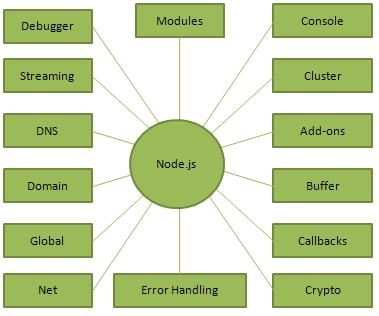
\includegraphics[width=\linewidth]{nodejs_concepts.jpg}
	 \caption{}
	 \label{fig:fig}
	
\end{figure}


\section{Where to Use Node.js?}
\begin{itemize}
\item I/O bound Applications
	
\item	Data Streaming Applications
	
\item Data Intensive Real-time Applications (DIRT)
	
\item	JSON APIs based Applications
	
\item	Single Page Applications	
\end{itemize}
\chapter{Environment Setup}
\section{444}
\chapter{First Application}
\chapter{Package Manager (NPM)}
\chapter{Callbacks Concept}
\chapter{Event Loop}
\chapter{Event Emitter}
\chapter{Buffers}
\chapter{streams}
\chapter{File System}
\chapter{Global Objects}
\chapter{Utility Module}
\chapter{Web Module}

\backmatter
% bibliography, glossary and index would go here.

\end{document}